
\section{Bandit Revenge}
Difficulty: Silver
\subsection*{Rules}
\textbf{Rulebound Cultist} - At the start of the players turn, place a flurry counter on the cultist. When a cultist dies, it uses all flurry tokens.
\subsection*{Story}

A new bandit has risen to prominence near the imperial capital. From the reports he is on some revenge quest for the death of his father. Many villages in the imperium centre have suffered during his search for those responsible. You are sent to investigate how the bandit could gather so much power so fast. As all reconnaissance must, you start by chasing down one of his raiding parties.


\subsection*{Encounter 1}

\begin{minipage}[t][10cm][t]{\textwidth}
	\centering
	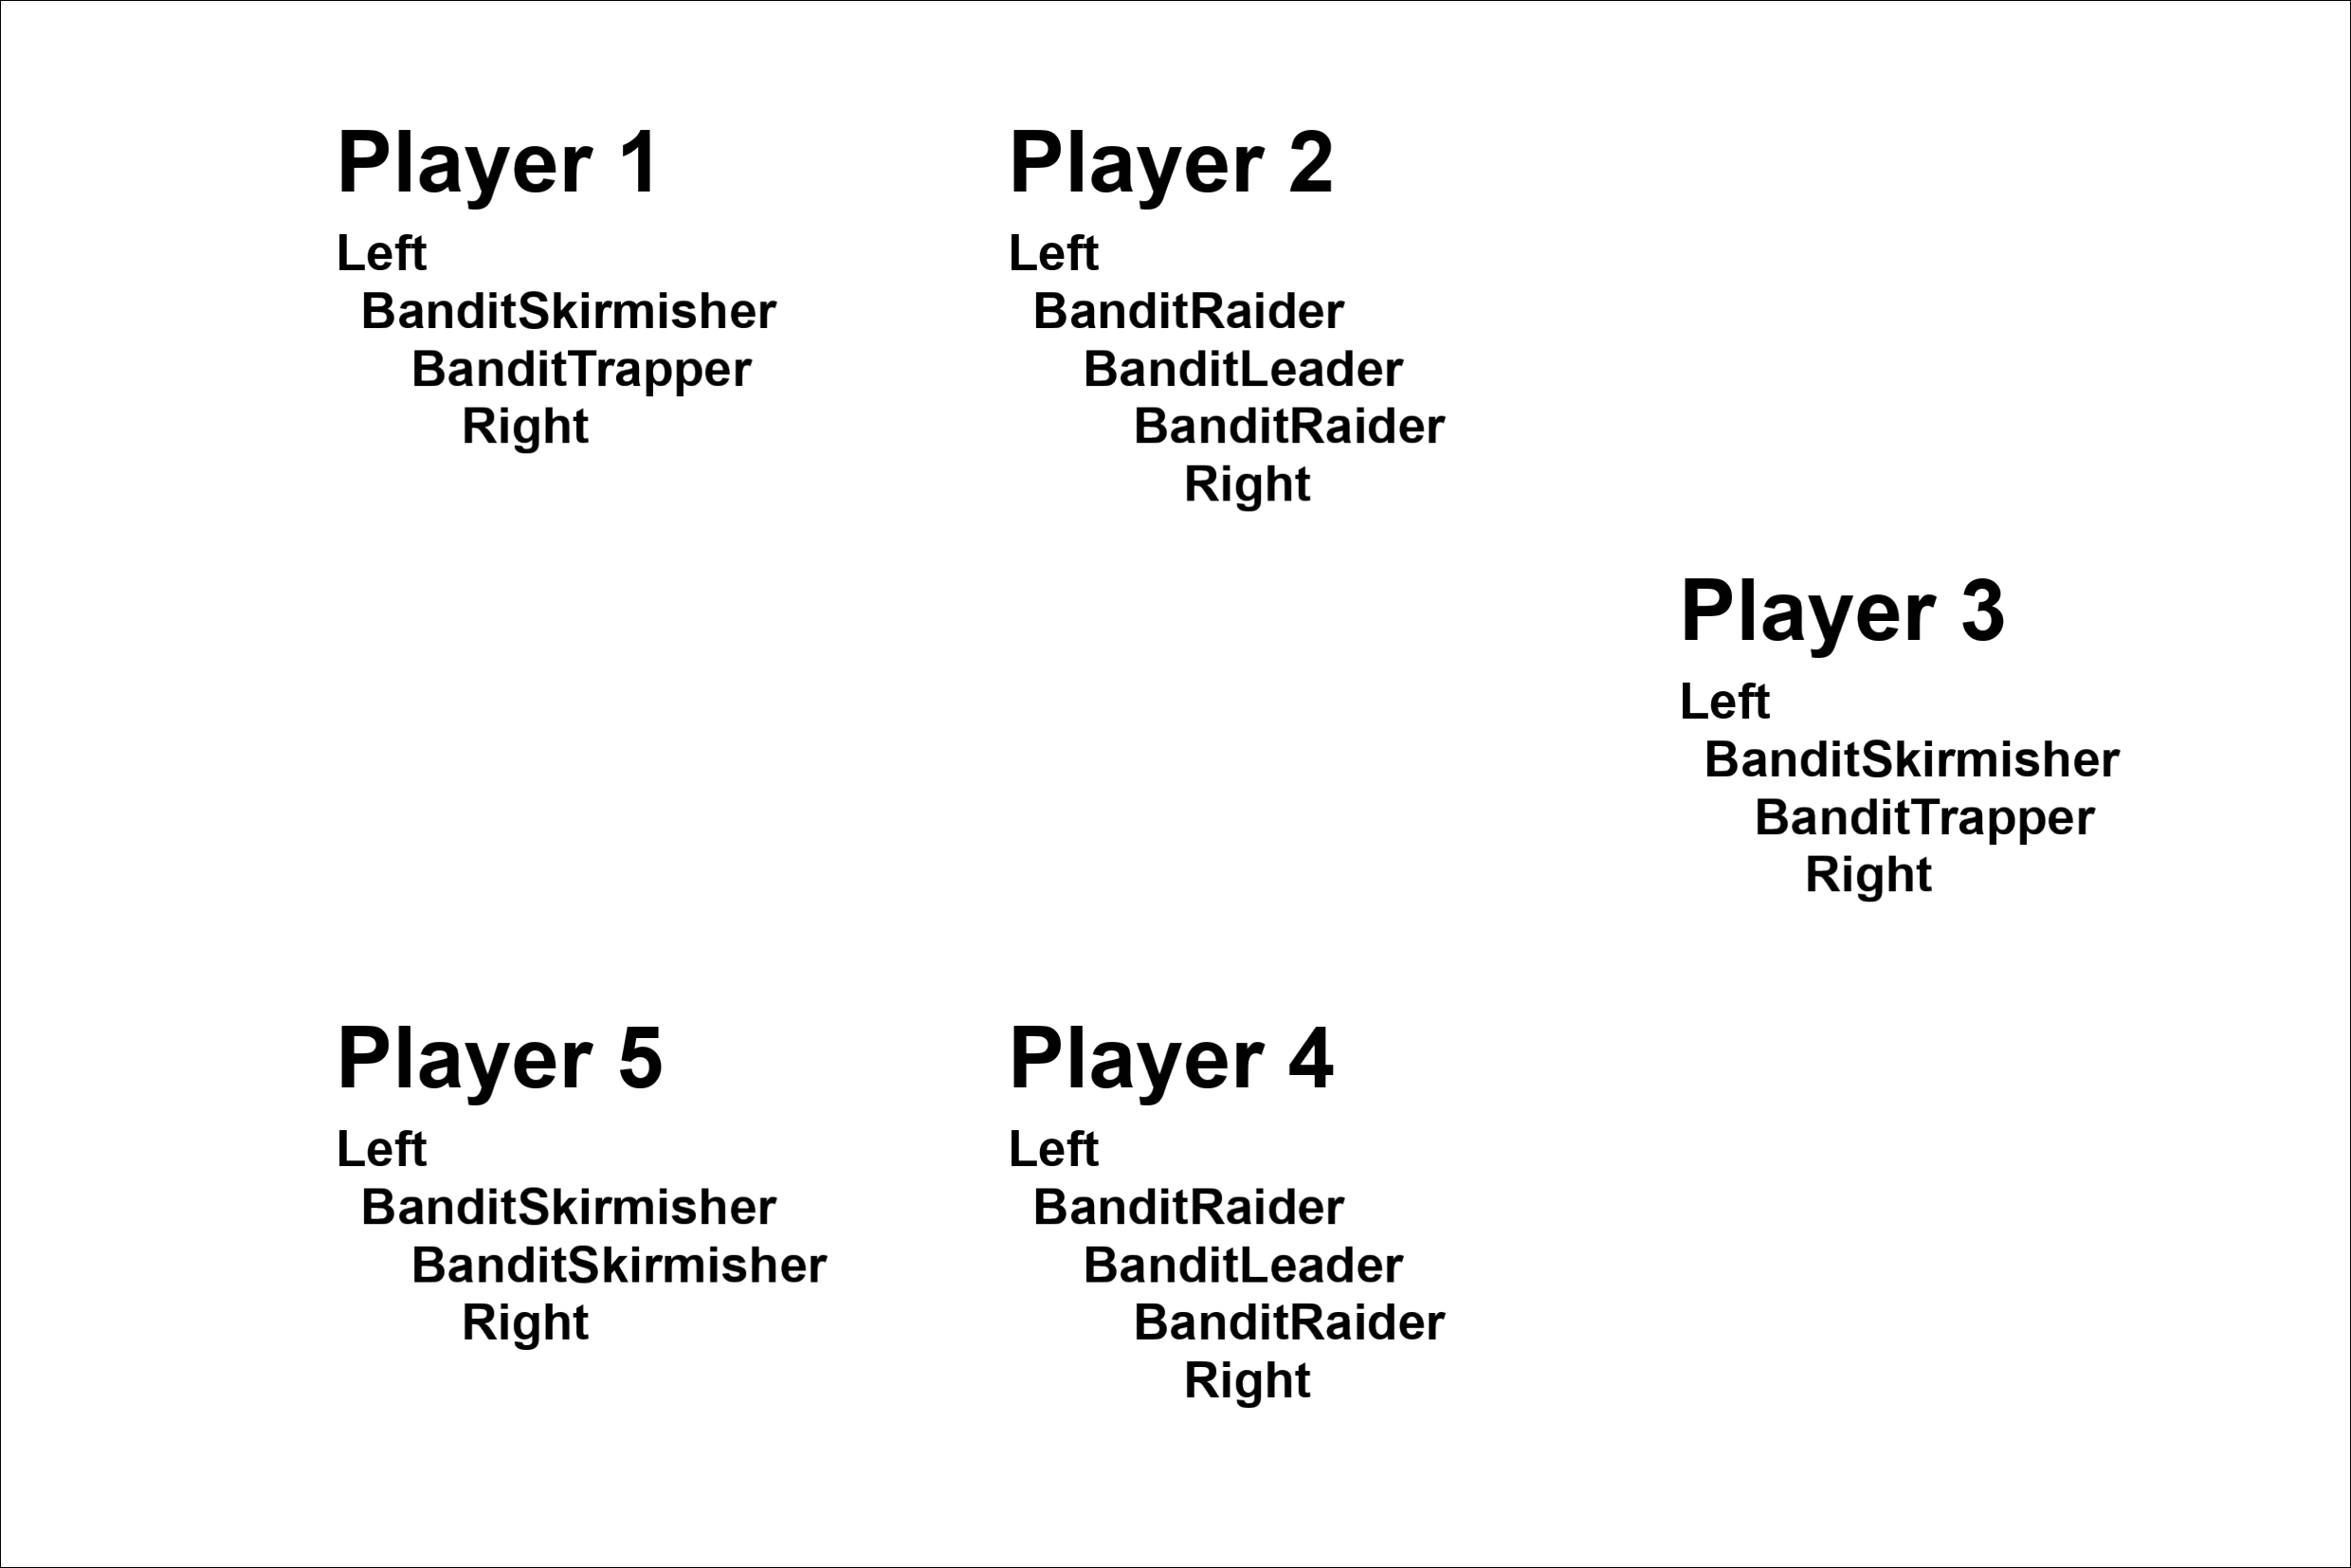
\includegraphics[width=0.8\linewidth, valign=t]{./Story5/Stories_13.png}
\end{minipage}


\subsection*{Draw an Event \& Level Up}

You interrogate the survivors about the whereabouts of their leader. It turns out he is situated near the hideout of your fist query, all the way back when you first started your adventures.
When you bust down the hideout, your suspicions are confirmed. The bandit leader immediately recognises you and lets out a roar of pure hatred. As he rushes you, the explanation for his sharp rise to notoriety becomes clear. The warlord employs necromancers and cultists.  It is time to put an end to this horrendous act against god, humanity and the imperium!

\newpage
\subsection*{Encounter 2}

\begin{minipage}[t][10cm][t]{\textwidth}
	\centering
	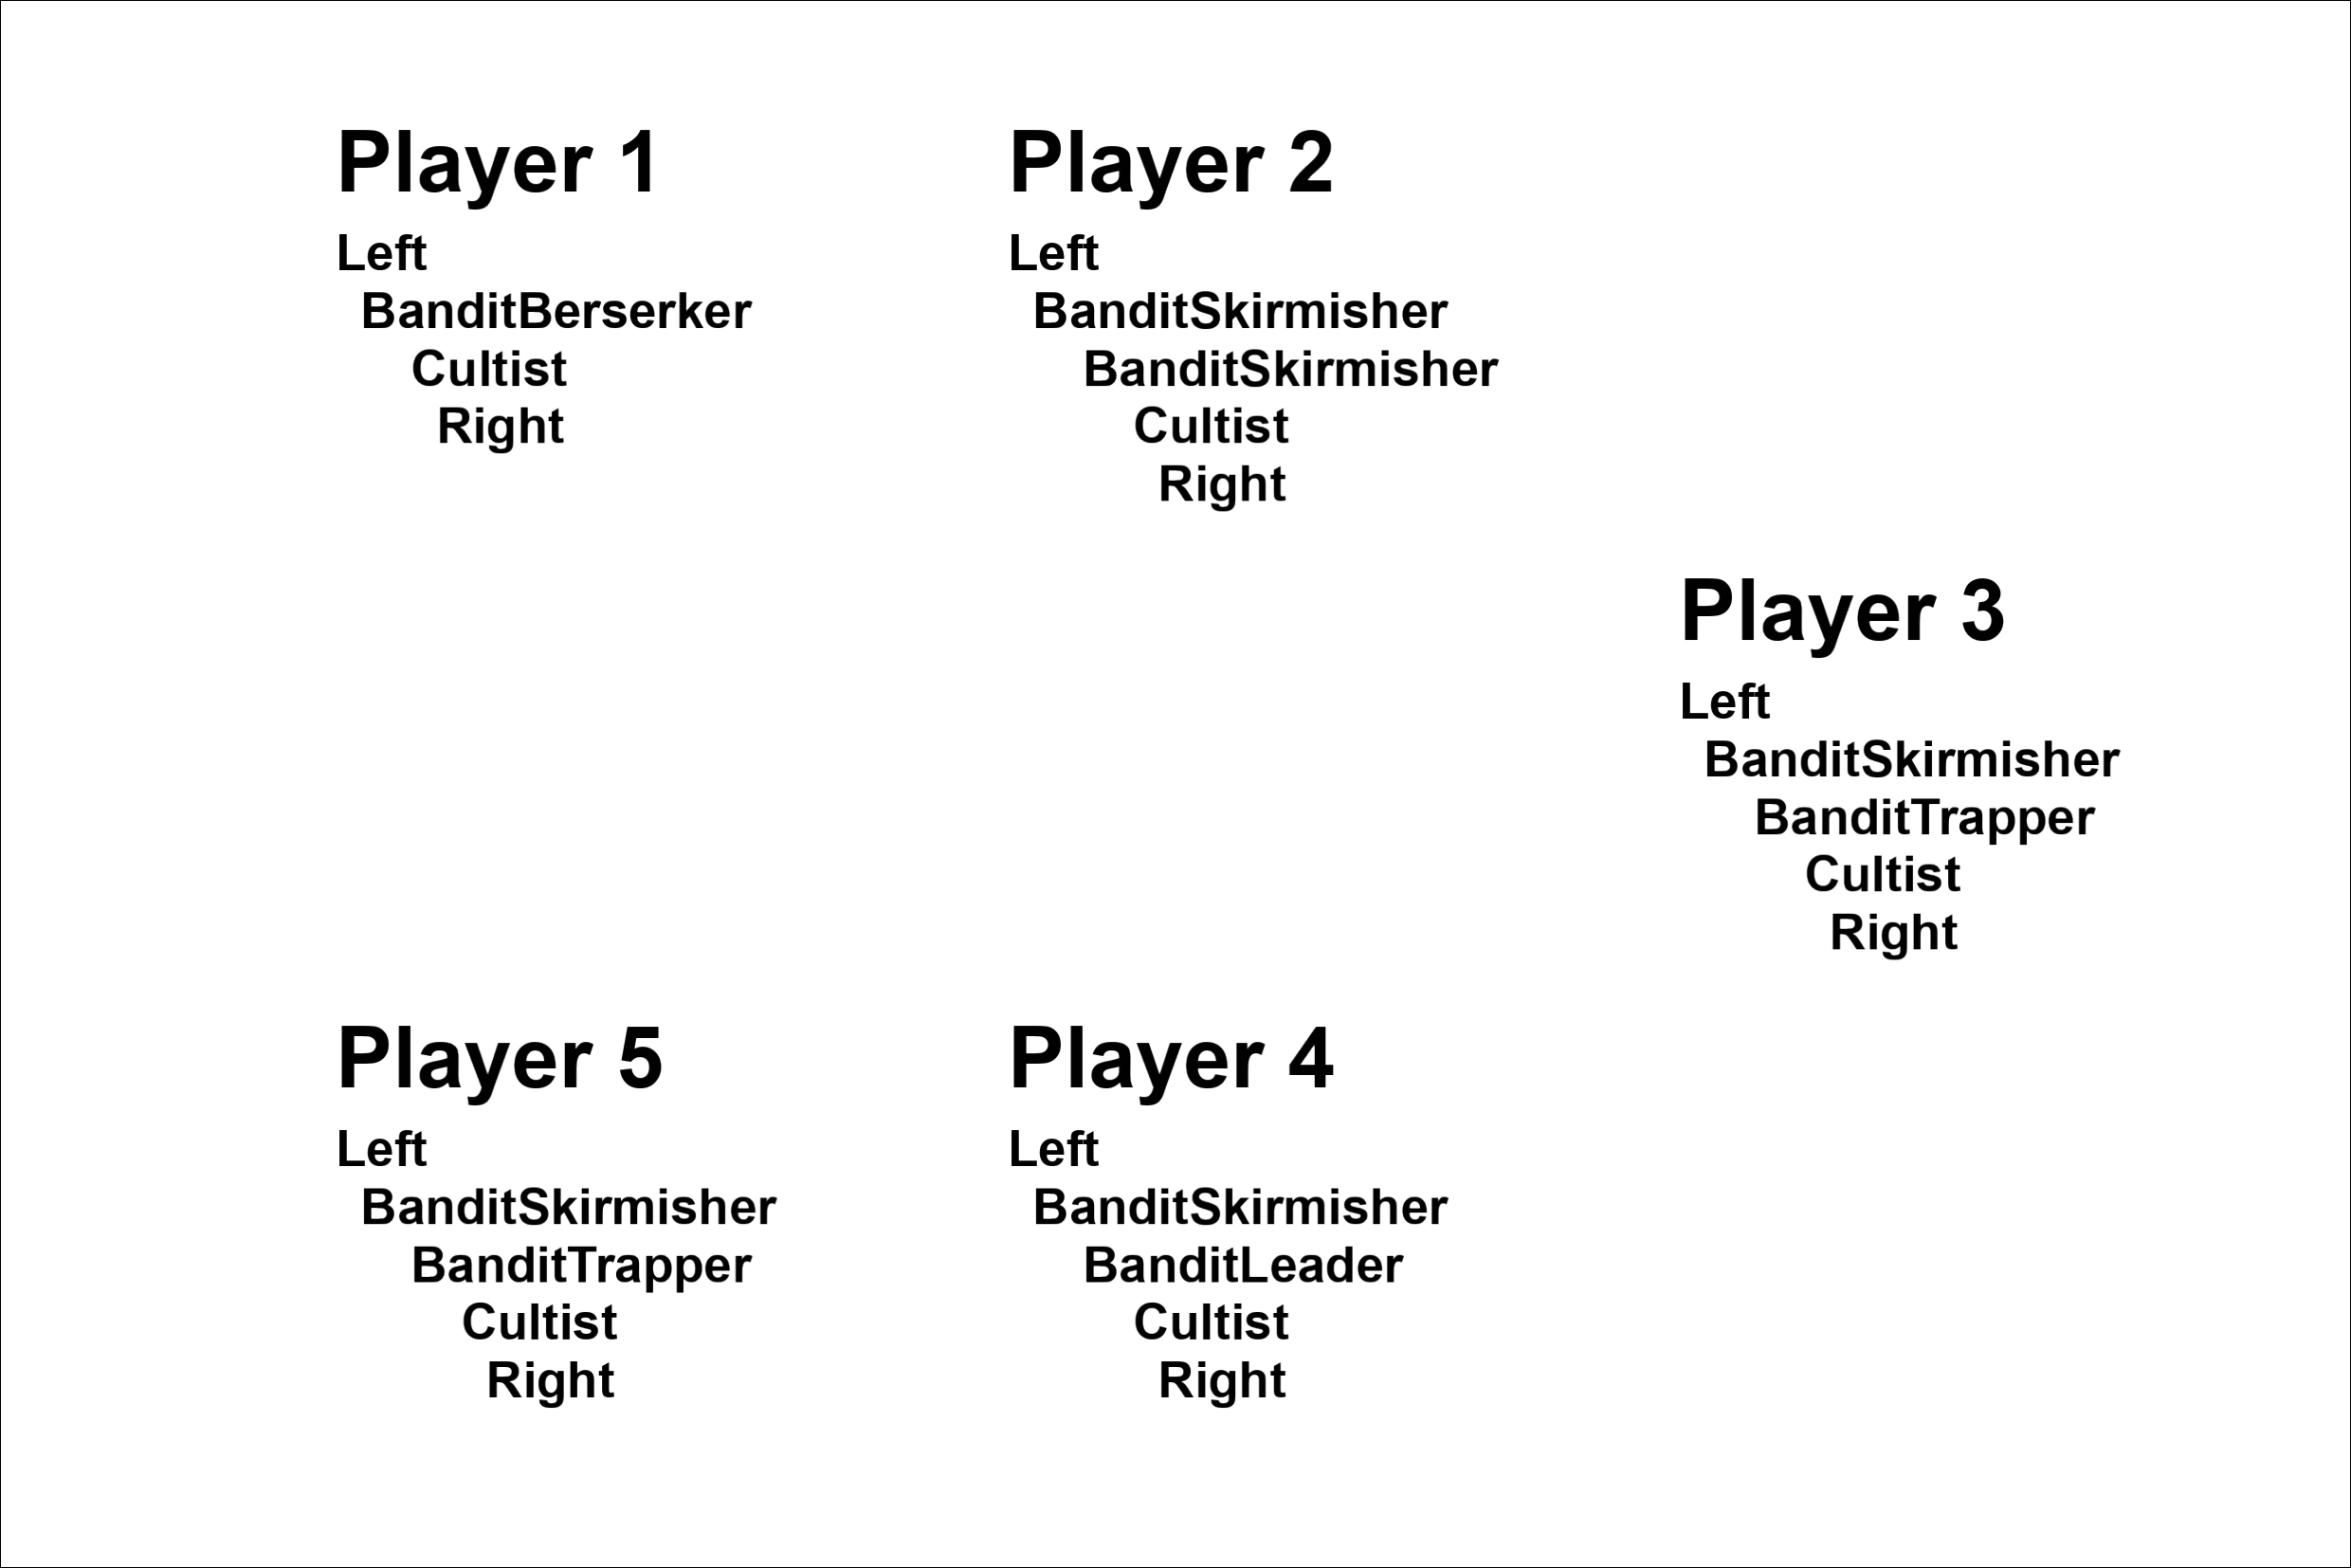
\includegraphics[width=0.8\linewidth, valign=t]{./Story5/Stories_14.png}
\end{minipage}

\subsection*{Draw an Event \& Level Up}

It seems the bandits has truly resolved to revenge at any cost. After you slay him, some zealous bandits tangle you up while the cultists drag him down the back to the basement.  After a short strategy meeting you proceed down the dimly lit stairs. The air is rank and humid, and otherworldly chants ring in your ears. When you finally arrive, you find that the ranks of the cultists are bolstered by the vengeful soul of the warlord and the remains of the bandits.


\subsection*{Encounter 3}


\begin{figure}[ht]
	\centering
	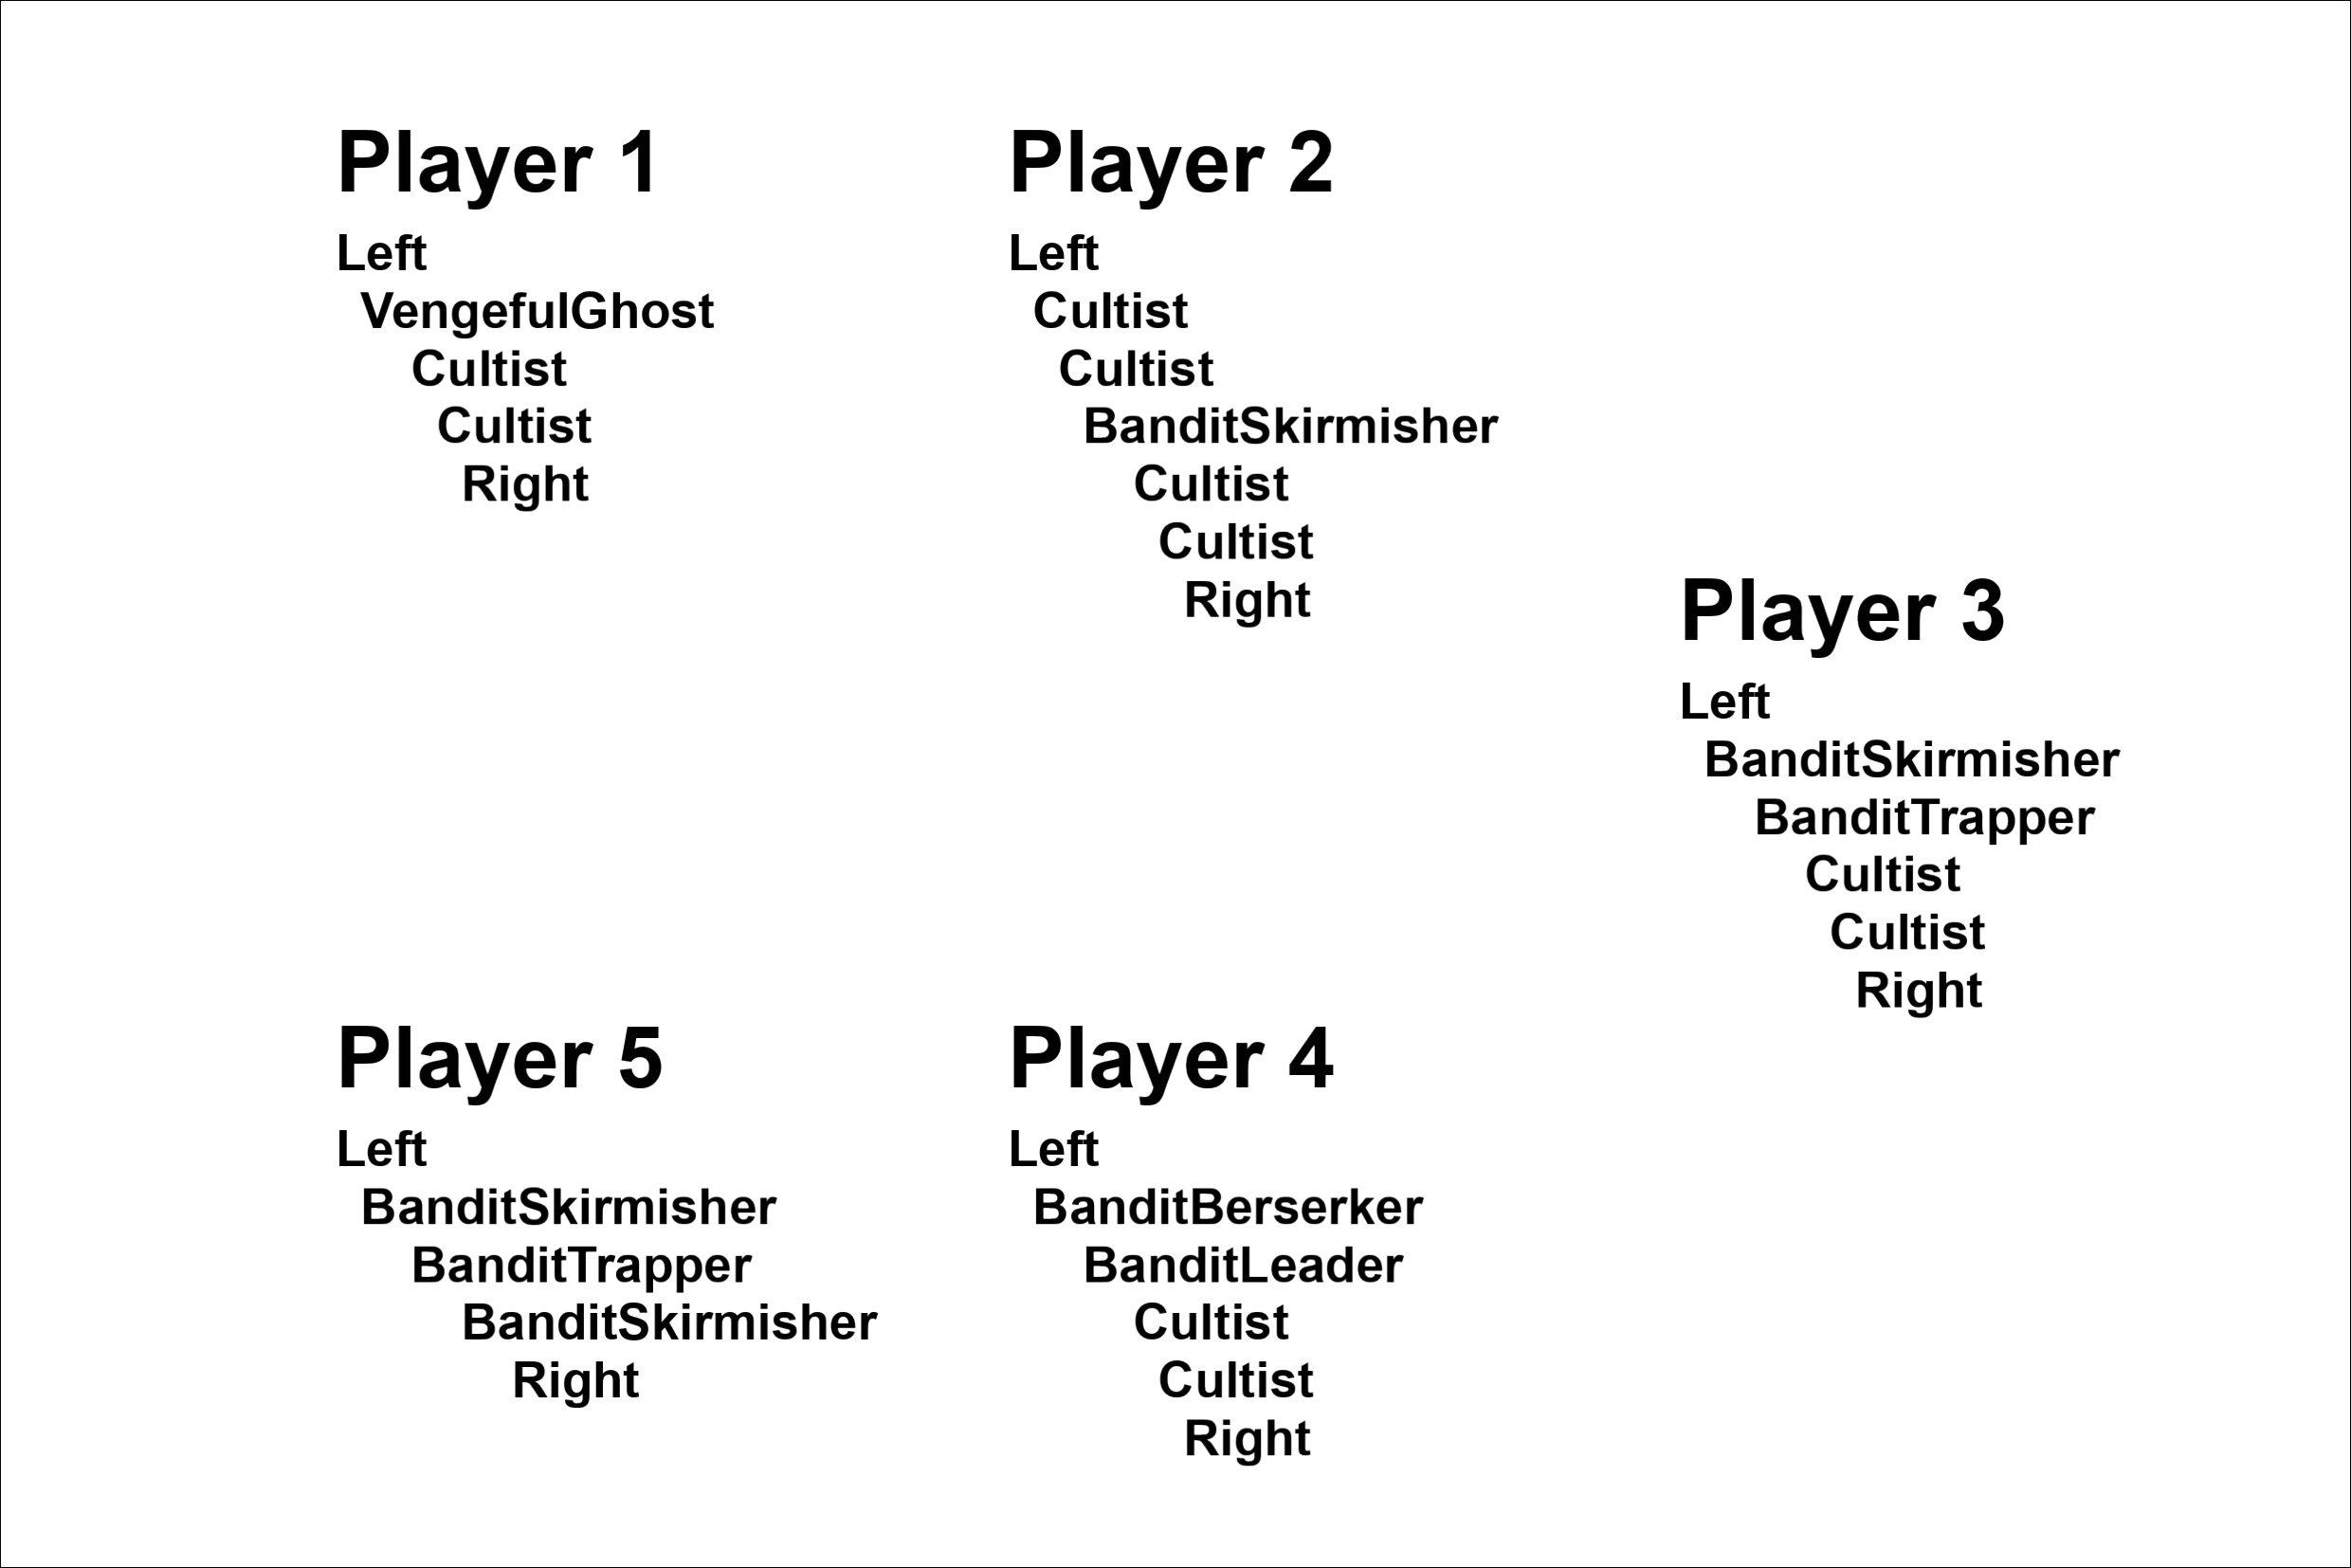
\includegraphics[width=0.8\linewidth, valign=t]{./Story5/Stories_15.png}
	
\end{figure}

You emerge victorious to a calm evening outside of the hideout. It is likely that no one will truly appreciate what you have to put on your adventures, but at least the villagers stay safe while you keep watch.
